\chapter{Hardware}
\lhead{Kapitel 4: \emph{Hardware}}

Der Kernpunkt der Bachelorarbeit ist die Analyse des DMX-Signals. Das Projekt wird für die Lehre eingesetzt, um das DMX Protokoll anschaulich und intuitiv zu erklären. Die Struktur des DMX Paketes soll daher heruntergebrochen und verständlich dargestellt werden.

Für die Signalverarbeitung und Bildschirmausgabe wird ein Raspberry Pi 4 in der 8 GB RAM Variante verwendet. Der Raspberry Pi 4, kann mithilfe einer Stiftleiste leicht mit externer Hardware kommunizieren.

Eine LED Matrix-Anzeige zeigt, und stellt das verarbeitete Signal dar. Es kann zwischen verschiedene Bildschirmanzeigen gewechselt werden, um verschiedene Aspekte des Protokolls genauer zu veranschaulichen. Die LED Matrix wird vom Raspberry Pi gesteuert. Allerdings wird eine Erweiterungsplatine, für den Raspberry Pi benötigt, um die LED Matrix direkt ansprechen zu können.

Das DMX-Signal wird als differenzielles (oder auch symmetrisches) Datensignal übertragen, um eine gute Rauschunterdrückung zu erhalten. Dieses symmetrische Datensignal wird in ein unsymmetrisches Datensignal gewandelt, um das Analysieren des Signals zu vereinfachen. Außerdem empfiehlt der DMX-Standard eine elektrische Isolierung zwischen dem DMX Bus und dem Rest der elektronischen Komponenten. Eine Platine wurde daher für dieses Projekt angefertigt.

Im Projekt arbeiten mehrere Komponenten zusammen, um das DMX-Signal zu verarbeiten und auf dem Bildschirm auszugeben. Die Elektronik muss von äußerlichen Einwirkungen geschützt werden. Im Projekt wurde dafür ein Gehäuse modelliert und mithilfe eines 3D-Druckers erstellt.

Für das Projekt ist es wichtig, das DMX-Signal zu analysieren und auch die genauen Zeitabstände abzugreifen. Dafür wird ein USB Logikanalysator benutzt. Das Signal kann mit bis zu 24 MHz aufgenommen werden.

\section{Raspberry Pi}
Der Raspberry Pi bietet ausreichend Rechenleistung für die benötigten Anforderungen. Ein Linux-Betriebssystem wird verwendet, um eine Vielzahl von bestehenden Bibliotheken zu benutzen. Es gibt bereits Bibliotheken für die Signalverarbeitung und für die Bildschirmausgabe, die im Projekt eingebunden werden können.

\section{LED-Matrix}

Für die Darstellung des Signals wird eine 64x64 LED Matrix \ref{fig:led_matrix} verwendet. Der Bildschirm kann gut aus mehreren Blickwinkeln betrachtet werden und ist groß genug, um ihn auch aus mehreren Metern Abstand gut sehen können. Dies ist erforderlich, da mehrere Studierende gleichzeitig auf den Bildschirm schauen werden.

\begin{figure}[H]
	\centering
	\begin{subfigure}{.32\textwidth}
		\centering
		
\includegraphics[width=\linewidth]{Pictures/LedMatrix}
		\caption{Led Matrix\cite[S.1]{JoyItLedMatrix}}
	\end{subfigure}	
	\begin{subfigure}{.32\textwidth}
		\centering
		\shadowimage[angle=-90,width=.93\linewidth]{Pictures/finishedProduct/dmxAnalyzer9}
		\caption{Spitzer Blickwinkel}
	\end{subfigure}	
	\caption{Gehäuse}
	\label{fig:led_matrix}
\end{figure}


Ein gepuffertes Signal für den Bildschirm ist wünschenswert, um ein mögliches Zerreißen des Bildes auf der LED Matrix zu vermeiden. Dafür wird eine handelsübliche Platine \ref{fig:led_matrix_steuer_platine} für den Raspberry Pi verwendet. Der Raspberry Pi kann mithilfe der Platine bis zu 4 Bildschirme hintereinander schalten und bis zu 3 Bildschirme parallel steuern. Daher können theoretisch bis zu 12 Bildschirme gleichzeitig angesteuert werden.

\begin{figure}[H]
	\centering
	\shadowimage[width=.3\linewidth]{Pictures/LedMatrixControllerPlatine}
	\caption{Raspberry Pi LED Matrix Erweiterungsplatine}
	\cite[S.1]{JoyItLedMatrix}
	\label{fig:led_matrix_steuer_platine}
\end{figure}

\section{Platine DMX Breakout}

Die DMX Spezifikation empfiehlt eine galvanische (elektrische) Trennung vom DMX Bus und dem Rest der Platine\cite[S.22]{DMX512-Protocol-Standard}. Die DMX Kabel können mehrere 100 Meter lange Signale weiterleiten. Elektrostatische Aufladungen, können die maximale spezifizierten Spannungen übersteigen. Eine elektronische Isolierung \ref{fig:DmxIsolation}, des Busses zu anderen Komponenten ist vorteilhaft, um mögliche Schäden zu minimieren.

\begin{figure}[H]
	\centering
	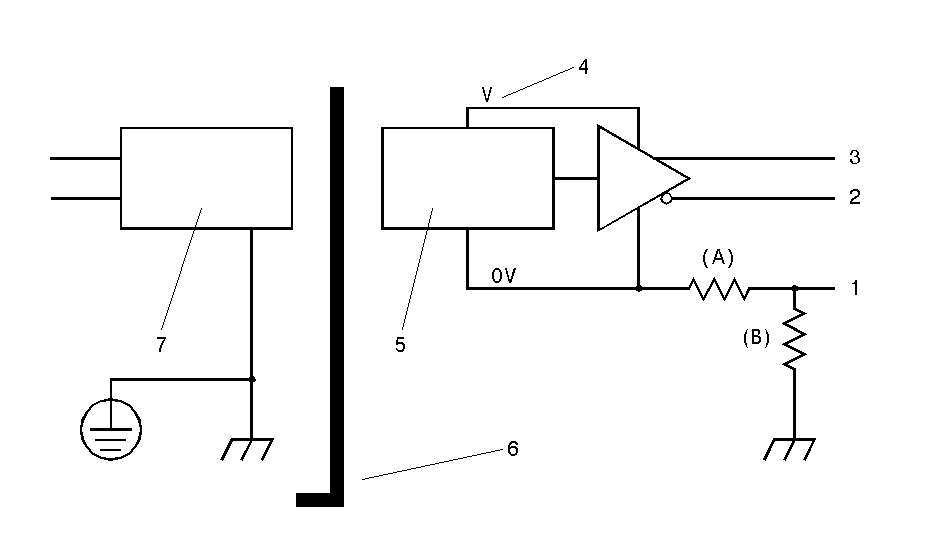
\includegraphics[width=0.5\linewidth]{Pictures/DmxIsolation}
	\caption{DMX elektrische Isolierung \cite[S.22]{DMX512-Protocol-Standard}}
	\label{fig:DmxIsolation}
\end{figure}

Das Datensignal  besteht aus einem symmetrischen Kabelpärchen. Dies hat den Vorteil, dass elektromagnetische Störeinflüsse, einen deutlich kleineren Einfluss auf die Übertragungsqualität haben. Der benutzte Logikanalysator benötigt, jedoch ein einzelnes, nicht symmetrisches Datensignal.

Für das Projekt wurde dafür eine eigene Platine entwickelt.  Im Schaltplan \ref{fig:DmxBreakoutSchematic} ist der Aufbau der Platine aufgeschlüsselt.

\begin{figure}[H]
	\centering
	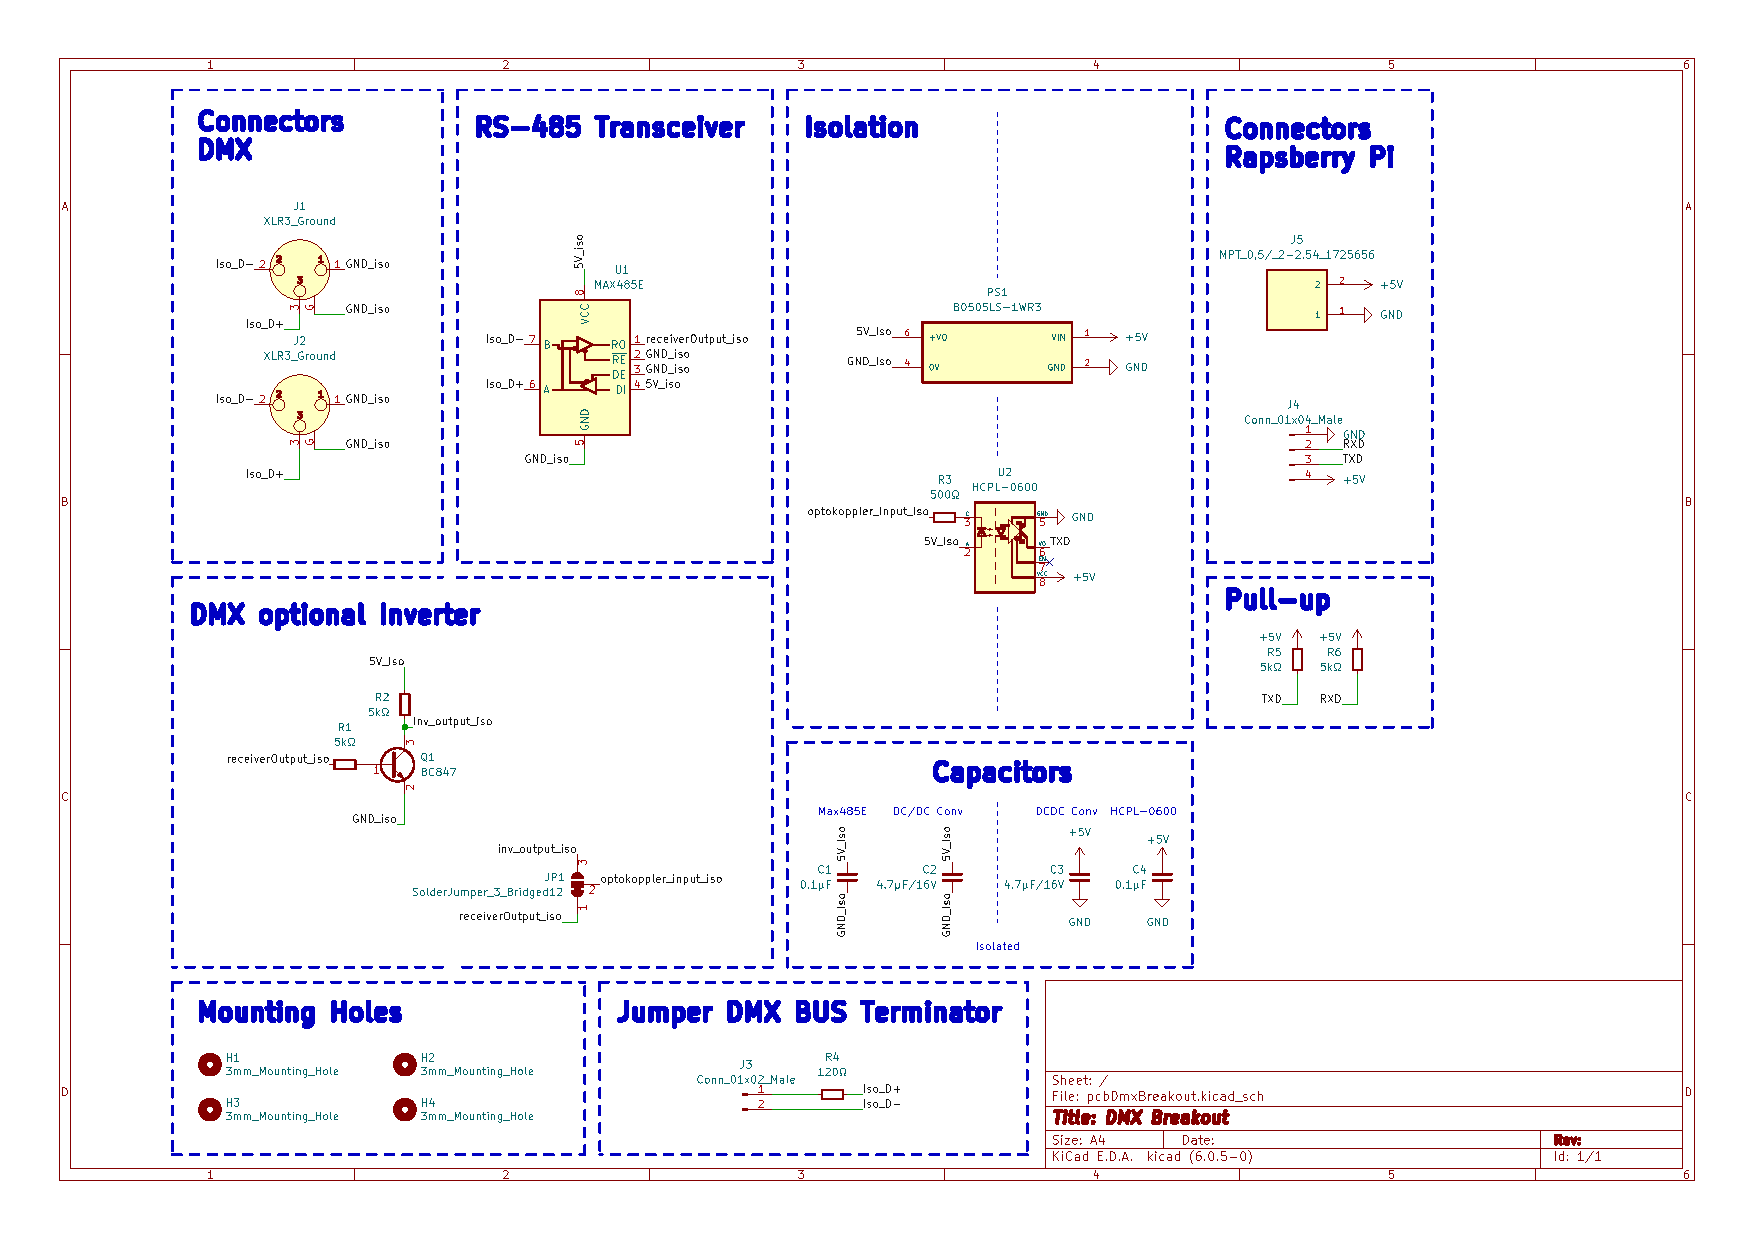
\includegraphics[width=1.0\linewidth]{Pictures/KicadPlatineSchematic}
	\caption{Schaltplan: DMX Platine}
	\label{fig:DmxBreakoutSchematic}
\end{figure}

Auf der linken Seite befinden sich die Eingänge. Das Signal wird in der Mitte verarbeitet und galvanisch getrennt. Auf rechten Seiten des Schaltplanes befinden sich die Ausgangssignale. Das symmetrische Signal wird mithilfe eines \emph{MAX485E RS-485 Transceiver} zu einem unsymmetrischen Signal gewandelt. Ein \emph{HCPL-0600 Optokoppler} wird verwendet, um die galvanische Trennung des Datensignals zu erreichen. Der blaue, gepunktete Strich in der Mitte des Schaltplans deutet auf die galvanische Trennung hin.

Die Belegung des XLR-Steckers für das DMX Datensignal, ist nicht bei allen Herstellern gleich.
Der Hersteller Martin Professionell hat bei alten Geräten vor dem Baujahr 2000 die symmetrischen Datensignale  "DMX+" und "DMX-" vertauscht.
Auch wenn nur noch wenige Geräte die Datensignale vertauschen, ist es trotzdem eine gute Vorgehensweise, auch diesen Fall zu berücksichtigen.
Dafür befindet sich ein DMX Inverter auf der Platine, der durch eine Lötbrücke, ein- oder ausgeschaltet werden kann.

Das Platinendesign ist im Aufbau \ref{fig:DmxBreakoutPcb} gezeigt.

\begin{figure}[H]
	\centering
	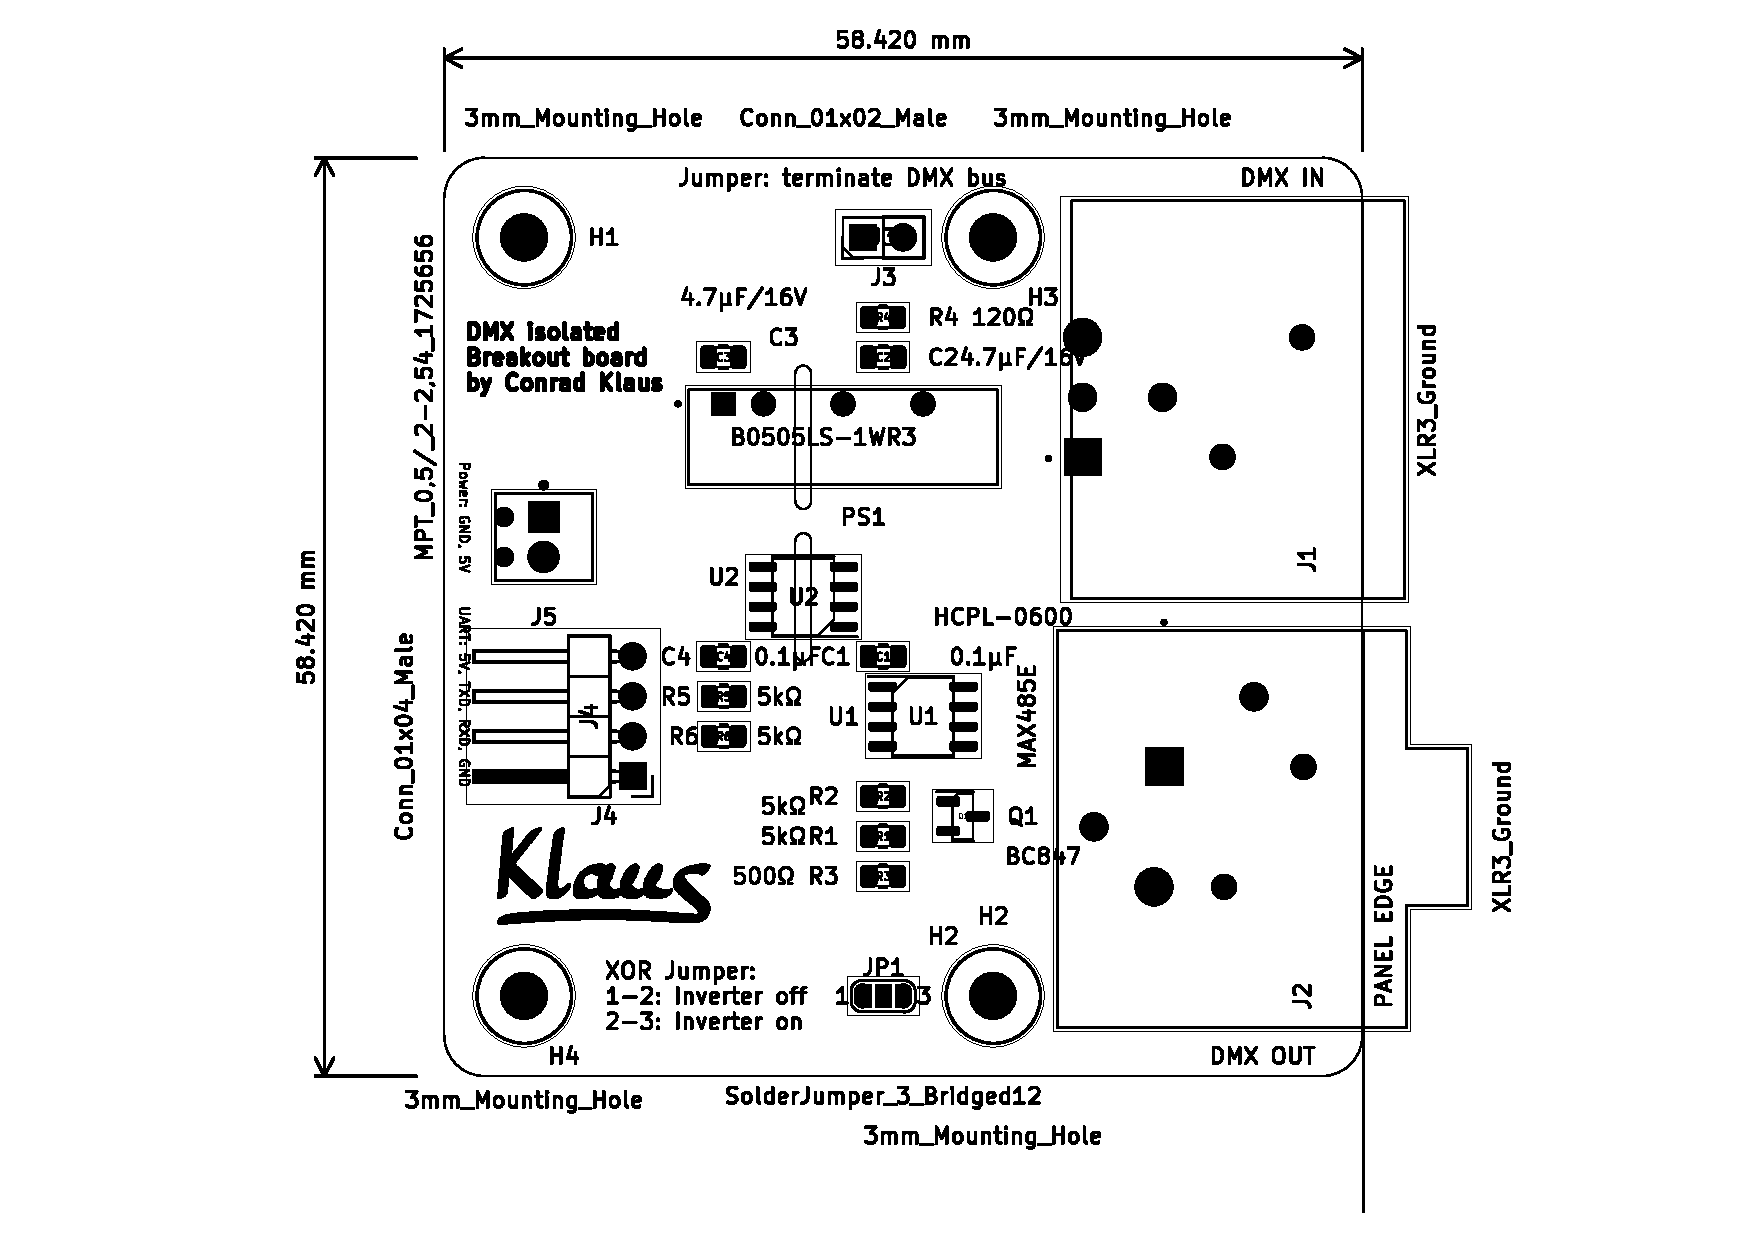
\includegraphics[width=0.8\linewidth]{Pictures/KicadPlatinePCB}
	\caption{Aufbau: DMX Platine}
	\label{fig:DmxBreakoutPcb}
\end{figure}

Die Platine \ref{fig:DmxBreakoutPcb} benötigt keine besonders starke elektromagnetisches Rauschunterdrückung. Trotzdem ist es empfehlenswert, gängige Vorgehensweisen einzuhalten, wenn diese keine wesentlichen Extrakosten verursachen.
Der Hersteller der Platinen, hatte ungefähr den gleichen Preis (bei dieser Platinengröße) für eine 2- oder 4-schichtige Platine. Bei einer 4-schichtigen Platine können zwei Schichten für die Masse genutzt werden, um eine dritte Schicht vor elektromagnetisches Rauschen zu schützen. Diese 3. Schicht wird zwischen den beiden Schichten mit der Masse eingeführt und befindet sich dadurch in einem Fahrradieschen Käfig. Die Platine basiert daher auf einem 4-schichtigen Entwurf, um das Datensignal des DMX Busses rauschfrei zu verarbeiten.

Die 3D gerenderte Platine \ref{fig:DmxBreakout3dView} zeigt den Aufbau mit den Komponenten.
\begin{figure}[H]
	\centering
	\hspace*{0.5cm}
	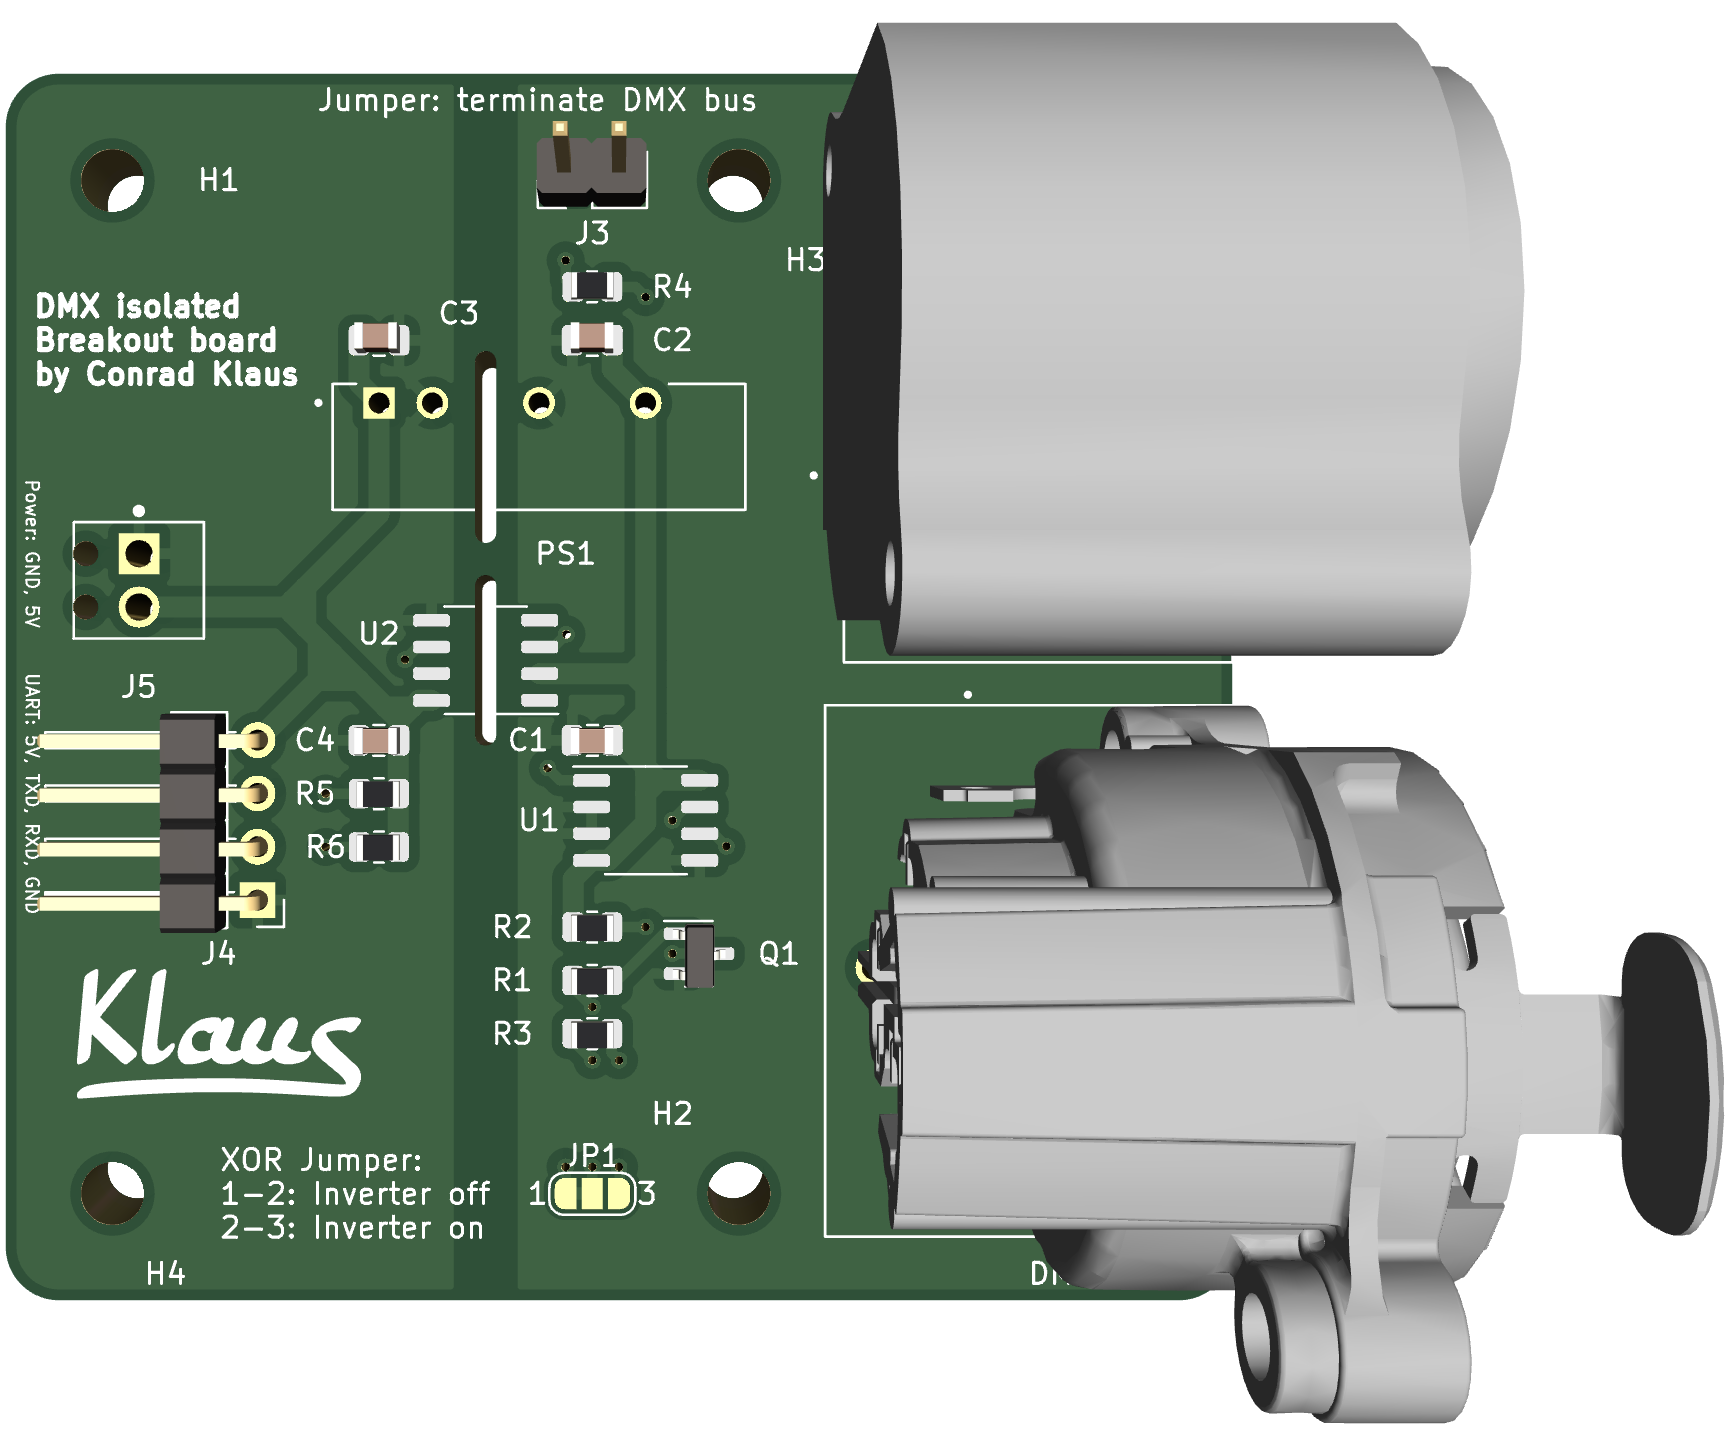
\includegraphics[width=0.5\linewidth]{Pictures/pcbDmxBreakout3dView}
	\caption{Aufbau mit Komponenten: DMX Platine}
	\label{fig:DmxBreakout3dView}
\end{figure}

Die elektrische Isolierung ist gut sichtbar. Alle Schichten sind in der Mitte unterbrochen. Der Optokoppler und der DC-DC Konvertierer, dienen für die Signalübertragung und Stromübertragung zwischen den isolierten Platinteilen. Unter den integrierten Schaltkreisen sind zusätzlich Aussparungen in der Platine eingebohrt, um die elektronische Isolierung zu verstärken.

\section{Logikanalysator}

Die Signalverarbeitung wird mithilfe eines handelsüblichen Logikanalysators \ref{LogicAnalyzer} umgesetzt. 

\begin{figure}[H]
	\centering
	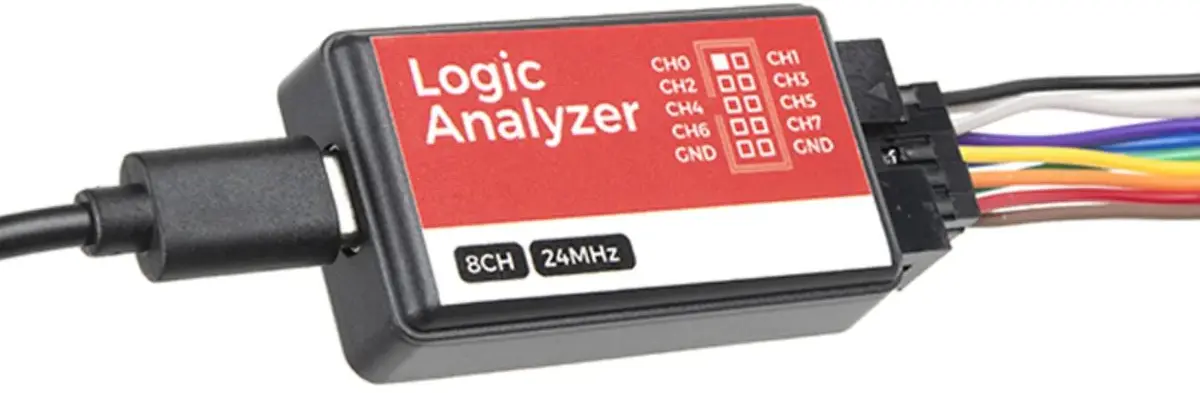
\includegraphics[width=0.6\linewidth]{Pictures/usb-logic-analyzer-side}
	\caption{Logikanalysator: MCU123 Saleae Logic Klone}
	\label{LogicAnalyzer}
\end{figure}


Die Vorgaben, für das Projekt, sehen vor, dass nicht nur der logische Inhalt des DMX Datenpakets entschlüsselt wird, sondern auch die exakten Zeitabstände zwischen den Signalflanken ausgelesen werden.

Neben der Verwendung des Logikanalysators wurden auch noch andere Optionen betrachtet: Die CPU könnte genutzt werden, um das Signal oft auszulesen und so das Signal aufzunehmen. Das verwendete Linux Betriebssystem ist jedoch kein Echtzeitbetriebssystem. Das bedeutet, dass nicht garantiert werden kann, dass das Signal kontinuierlich ausgelesen wird, da das Betriebssystem zu jedem Zeitpunkt ein anderes Programm, die CPU Zeit zuweisen kann. Eine Möglichkeit, um dies zu umgehen, wäre es den Prozess über das Betriebssystem auf einem Kern zu fesseln. Tatsächlich macht dies der Treiber für die Bildschirmsteuerung bereits. Noch einen weiteren Kern nur für das Auslesen, des Signals zu blockieren, würde die Geschwindigkeit des Raspberry Pi stark verlangsamen. Der Raspberry Pi 4 hat insgesamt 4 Kerne. Die Hälfte der CPU Kerne zu blockieren, ist sehr Ressourcen verschwenderisch.

Eine weitere Überlegung war es den Raspberry Pi Pico zu verwenden: Der Raspberry Pi Pico, ist im Gegensatz zum Raspberry Pi 4 ein Mikrocontroller. Dieser besitzt eine programmierbare Ein- und Ausgangs Peripherie (\emph{Programmalbe Input Output - PIO}). Diese Peripherie kann genutzt werden, um Signale per Hardware in Echtzeit zu verarbeiten. Eine Möglichkeit wäre es, die Bits in den RAM zu schreiben, und diese dann im Programm auszulesen \cite[S. 43]{RPiPicoPIO}. Auf dem Pico läuft jedoch kein richtiges Betriebsystem, da er ein Mikrocontroller ist. Daher würden viele Bibliotheken, wie z.B. der Bildschirmtreiber, der Signaldecoder und viele Rust Bibliotheken nicht mehr funktionieren. Daher ist auch diese Option nicht geeignet.

Auch würde überprüft, ob die UART Schnittstelle des Raspberry Pi 4 verwendet werden kann, weil das DMX Signal im Wesentlichen aus einem UART Signal besteht. Für die Markierung des Anfanges eines DMX Paketes wird, das UART Protokoll jedoch abgewandelt, um ein Pause- und ein \emph{MarkAfterBreak} Signal einzubinden. Der Raspberry Pi kommt leider nicht mit dieser Abwandlung zurecht\cite[S.20]{RaspberryPiDmxInterface}. Die UART Schnittstelle, bietet auch keine Möglichkeit, um den zeitlichen Ablauf des Signals nachzuvollziehen. Die UART Schnittstelle kann deswegen auch nicht für die Signalabtastung verwendet werden.

Eine weitere Möglichkeit, ist die SPI (\emph{Serial Peripheral Interface}) Schnittstelle des Raspberry Pi. Das Signal kann mit dem Raspberry Pi 1 mit bis zu 2 MHz aufgenommen werden \cite{RaspberryPiDmxInterface}[30].

Diese Option lässt aber einige Fragen auf. Das DMX Signal kann oft nicht komplett aufgenommen werden. Möchte man immer das komplette DMX Signal aufnehmen, ist nur noch eine Abtastrate von 1 MHz möglich. Der Raspberry Pi 4 kann insgesamt 65536 ($2^{16}$) Abtastungen aufnehmen. Ein komplettes DMX Signal ist min. 22,624 ms lang\cite{DMXWikiTiming}. Wenn wir immer ein komplettes Signal aufnehmen wollen, müssen wir $  \SI{22.624}{\ms}
 * 2 \approx \SI{50}{\ms}$ aufnehmen.



Berechnen wir nun die maximale Aufnahmegeschwindigkeit für den Raspberry Pi ist dies:
\[\frac{\SI{65536}{Abtastungen}}{\SI{50}{\ms}} \approx \SI{1.3}{\mega\hertz}\]
Die zeitliche Auflösung beträgt daher:
\[ \frac{1}{\SI{1.3}{\mega\hertz}} \approx \SI{760}{\ns}\]
Das DMX Protokoll besteht überwiegend aus dem UART Protokoll mit einer Übertragungsgeschwindigkeit von $250 \frac{\SI{}{\kilo\bit}}{\SI{}{\s}}$. Das bedeutet die Übertragungslänge eines Bits beträgt 4 us \cite{DMXWikiTiming}.

Mit unserer Abtastrate können wir ca. 5 Abtastungen pro Bit aufnehmen:
\[\frac{\SI{4}{\us}}{\SI{760}{\ns}} \approx 5\]

Für die genaue zeitliche Analyse sind jedoch mehr Abtastungen pro Bit wünschenswert. Deswegen ist auch diese Option nicht ausreichend. Außerdem, wäre diese Lösung, spezifisch für den Raspberry Pi 4. Ältere oder zukünftige Modelle könnten andere Hardwarekonfigurationen benötigen. Das Programm würde dann bei diesen Modellen ggf. nicht laufen.

Der USB Logik Analysator kann bis zu 24MHz aufnehmen. Diese Auflösung ist für unseren Zweck optimal. Die zeitliche Auflösung beträgt:
\[ \frac{1}{\SI{24}{\mega\hertz}} \approx \SI{42}{\ns}\]

Das bedeutet wir können ca. 96 Samples pro Bit aufnehmen:
\[\frac{\SI{4}{\us}}{\SI{42}{\ns}} \approx 96\]

Diese Auflösung ist gut geeignet.


\section{Gehäuse}

Das Projekt soll mobil, einfach aufzubauen und robust gegenüber äußerlichen Einwirkungen sein. Im Idealfall kann die verwendete Hardware direkt ins Gehäuse integriert werden. Für dieses Projekt wurde das Gehäuse daher in einer CAD Software modelliert und anschließend mithilfe eines 3D-Druckers produziert.

Die gerenderte Seiten- und Topansicht \ref{DmxCaseRender} zeigt den Aufbau des Gehäuses ohne die Abdeckung. 
\begin{figure}[H]
	\centering
	\begin{subfigure}{.5\textwidth}
		\centering
		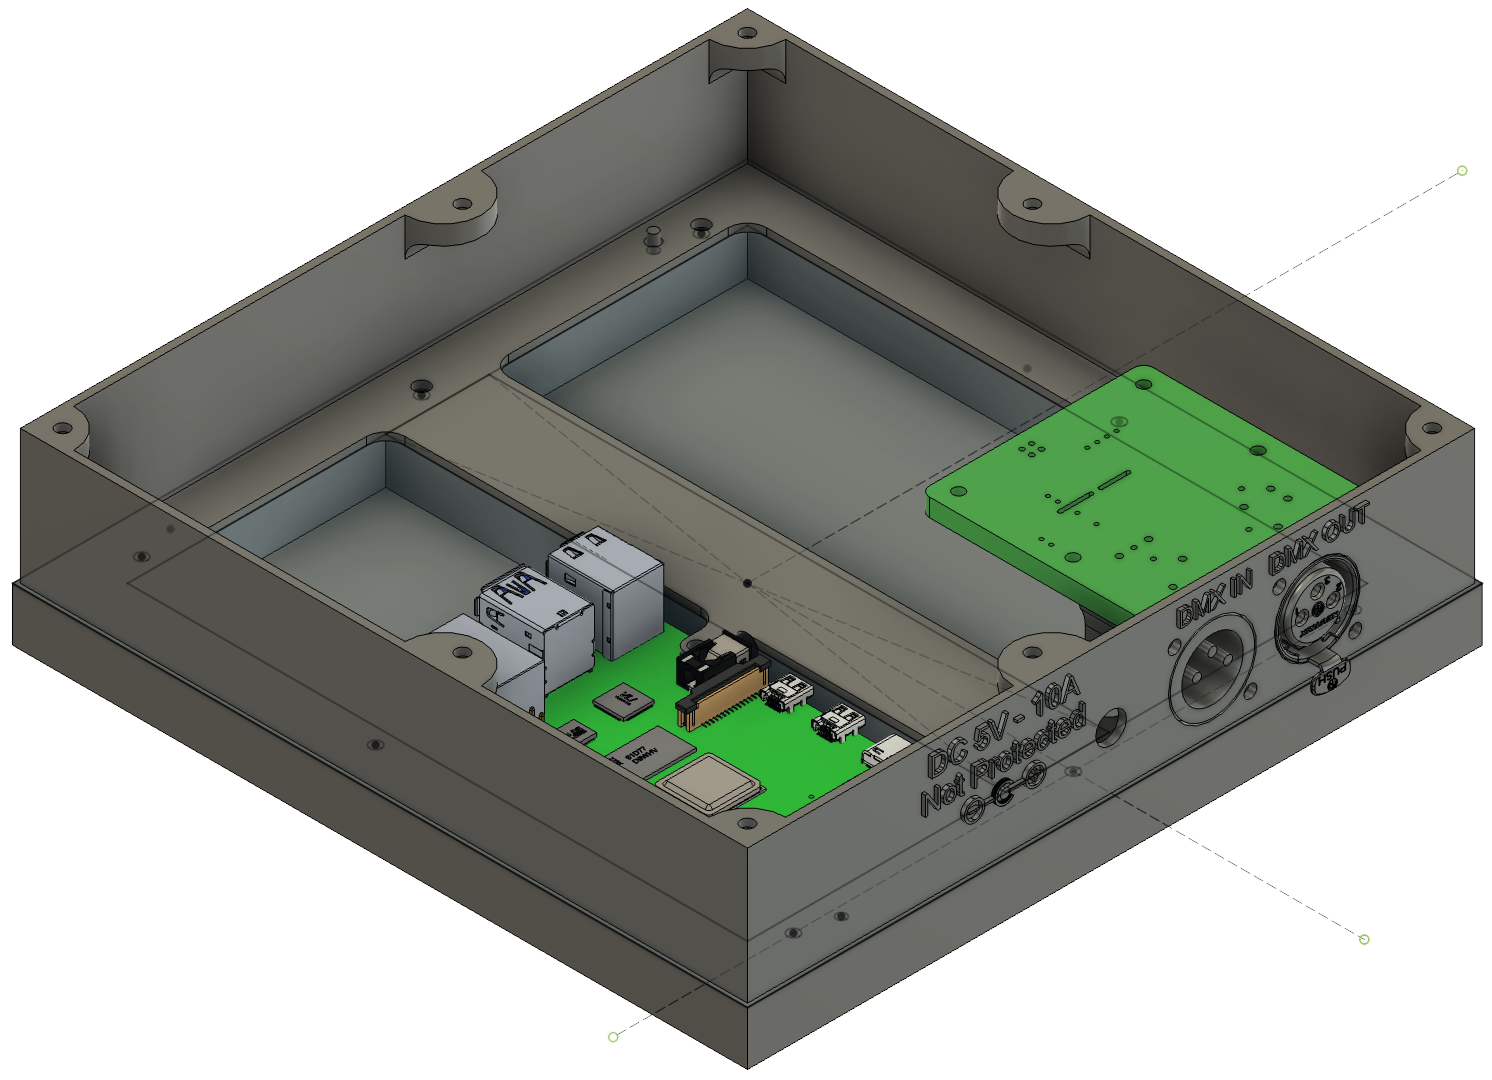
\includegraphics[width=0.9\linewidth]{Pictures/DmxCaseSideways}
		\caption{Seitenansicht}
		\label{DmxCaseSideViewRender}
	\end{subfigure}%
	\begin{subfigure}{.5\textwidth}
		\centering
		\shadowimage[width=0.9\linewidth]{Pictures/DmxCaseTop}
		\caption{Sicht von oben}
	\end{subfigure}
	\caption{DMX Analysator Gehäuse}
	\label{DmxCaseRender}
\end{figure}

Die LED Matrix befindet sich in der Seitenansicht \ref{DmxCaseSideViewRender} unter dem Gehäuse. Die LED Matrix kann direkt an das Gehäuse geschraubt werden, um einen nahtlosen Übergang zwischen Bildschirm und Gehäuse zu erzeugen. Die exakten CAD-Zeichnungen \cite[S.1]{LedMatrixCadDrawings} der LED Matrix haben dies ermöglicht.

Auch der Raspberry Pi kann direkt ins Gehäuse verschraubt werden. Der Raspberry Pi schwebt so in der Aussparung der LED Matrix. Das Gehäuse ist dadurch etwas flacher. Die DMX Platine kann direkt in der Seitenwand verschraubt werden. Alle Datensignale und auch die Steckverbindungen für die Stromversorgung, befinden sich auf einer Seite, um den Anschluss des DMX Analysators möglichst einfach zu halten. Neben dem Stromanschluss befinden sich auf der Seitenwand auch die benötigte Spannung und Stromstärke sowie eine Beschreibung der Polarität des Stromanschlusses. Das Gehäuse ist breit genug, damit es ohne externe Stützen stabil stehen kann. 

Die CAD-Zeichnungen beinhaltet nicht die Verkabelung der einzelnen Komponenten. Die Abbildung \ref{fig:DmxCaseWiring} zeigt den Strom- und Datenkabelaufbau.

\begin{figure}[H]
	\centering
	\begin{subfigure}{.32\textwidth}
		\centering
		\shadowimage[angle=-90,width=.93\linewidth]{Pictures/finishedProduct/dmxAnalyzer5}
		\caption{Verkabelung}
	\end{subfigure}
	\hfill
	\begin{subfigure}{.32\textwidth}
		\centering
		\shadowimage[angle=-90,width=.93\linewidth]{Pictures/finishedProduct/dmxAnalyzer7}
		\caption{USB Logikanalysator}
	\end{subfigure}
	\hfill
	\begin{subfigure}{.32\textwidth}
		\centering
		\shadowimage[angle=-90,width=.93\linewidth]{Pictures/finishedProduct/dmxAnalyzer6}
		\caption{Ein- und Ausgänge}
	\end{subfigure}
	\caption{Verkabelung}
	\label{fig:DmxCaseWiring}
\end{figure}

Für die Modellierung wurde Fusion360 benutzt. Fusion 360 verwendet einen parametrische Modellierungsansatz. Die Modellierung ist dabei von vorher definierten Merkmalen und Einschränkungen abhängig. Dabei können Skizzen mithilfe mathematischer Beziehungen erstellt werden und ein 3 dimensionales Model aufgebaut werden. Der Vorteil der parametrischen Modellierung ist, dass definierte Merkmale (wie z.B. die Wanddicke), im späteren Verlauf verändert werden können, und alle darauf aufbauenden Merkmale neu errechnet werden. 

Das Gehäuse wird von einer verschraubbaren Abdeckung \ref{DmxCaseLidRender} von äußerlichen Einflüssen geschützt. Das zusammengesetzte Projekt mit der LED Matrix und der DMX Gehäuse Abdeckung ist der Abbildung \ref{fig:DmxCase} zu sehen.

\begin{figure}[H]
	\centering
	\begin{subfigure}{.32\textwidth}
		\centering
		\shadowimage[angle=-90,width=.93\linewidth]{Pictures/finishedProduct/dmxAnalyzer1}
		\caption{Seitenansicht}
	\end{subfigure}
	\begin{subfigure}{.32\textwidth}
		\centering
		\shadowimage[angle=-90,width=.93\linewidth]{Pictures/finishedProduct/dmxAnalyzer8}
		\caption{Abdeckung}
	\end{subfigure}
	\begin{subfigure}{.32\textwidth}
		\centering
		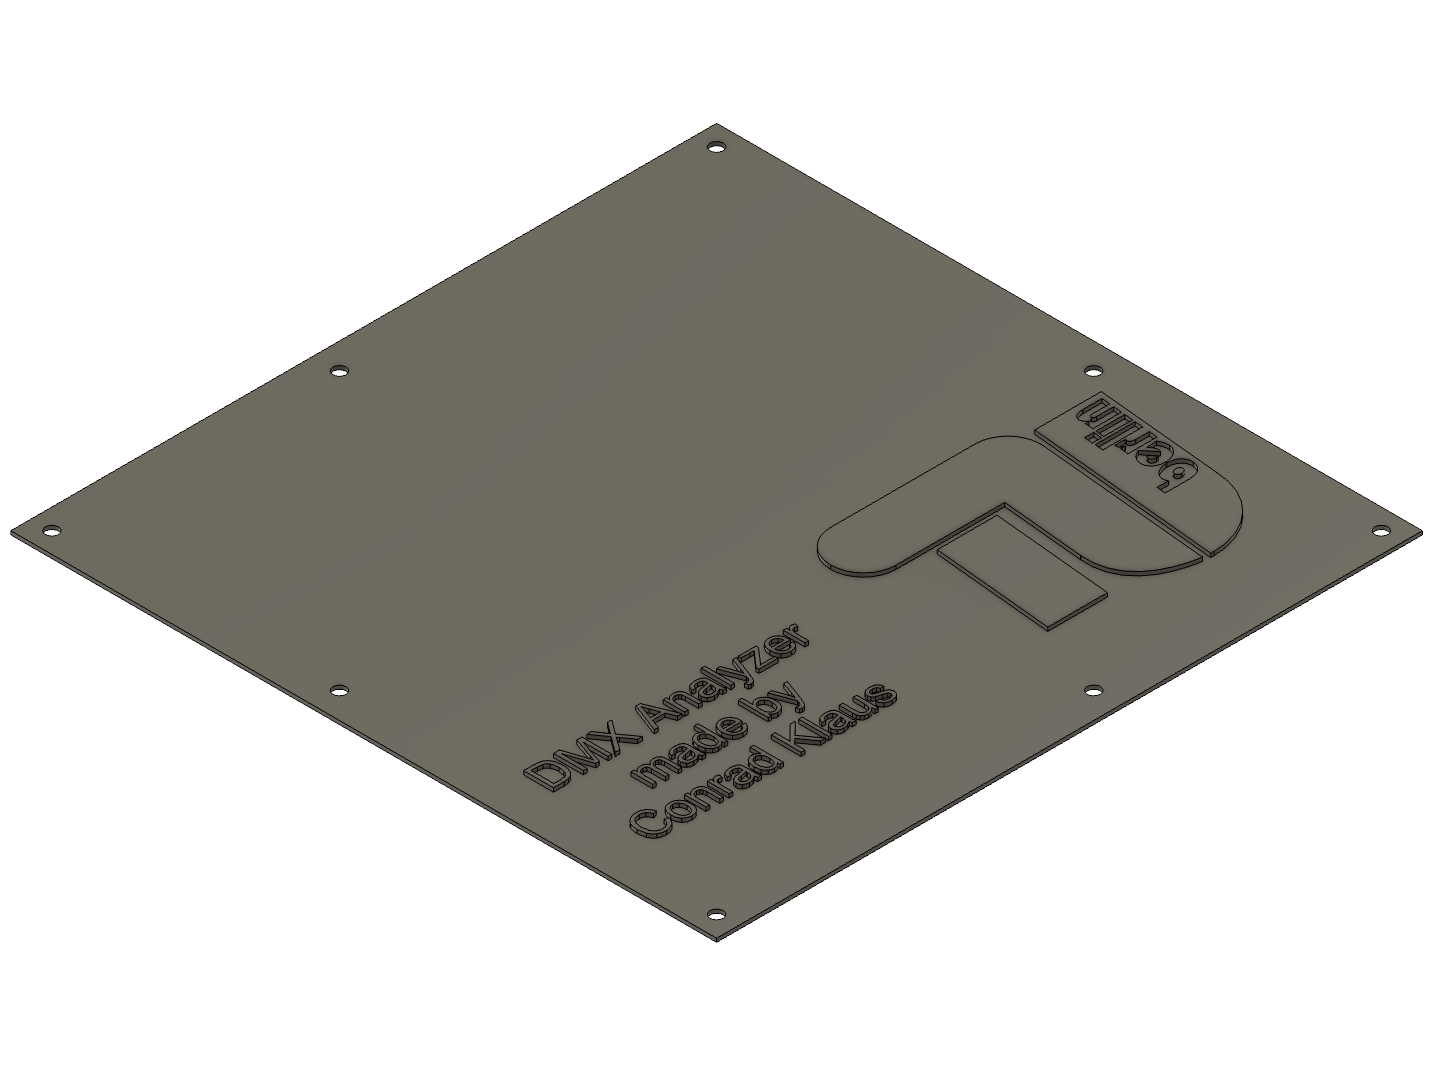
\includegraphics[width=\linewidth]{Pictures/DmxCaseLid}
		\caption{Abdeckung CAD Modell}
		\label{DmxCaseLidRender}
	\end{subfigure}
	\caption{Gehäuse}
	\label{fig:DmxCase}
\end{figure}

